\documentclass[margin=5pt]{standalone}
\usepackage[utf8]{inputenc}
\usepackage{tikz}
\usepackage{circuitikz}
\usetikzlibrary{circuits.logic.US}
%
\begin{document}
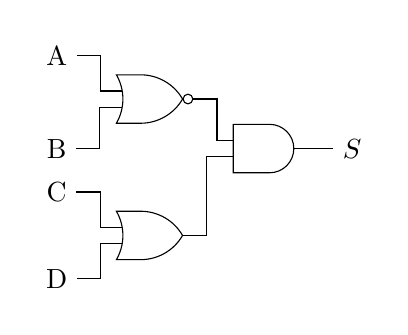
\begin{tikzpicture}[circuit logic US]
    %\node[] at (0,3) { $S = \overline{A + B} \cdot (C + D)$};
    %
    \matrix[column sep=5mm]{
        \node (iA)  {A}; &                                                   &\\
                         & \node [nor gate, logic gate inputs=nn] (nor1) {}; &\\
        \node (iB)  {B}; &                                                   & \node [and gate] (and1) {}; & \node (out) {$S$};\\
        \node (iC)  {C}; &                                                   & \\
                         & \node [or gate, logic gate inputs=nn] (or1) {};   & \\
        \node (iD)  {D}; &                                                   & \\
    };
    %
    \draw (iA.east) -- ++(right:3mm) |- (nor1.input 1);
    \draw (iB.east) -- ++(right:3mm) |- (nor1.input 2);
    \draw (iC.east) -- ++(right:3mm) |- (or1.input 1);
    \draw (iD.east) -- ++(right:3mm) |- (or1.input 2);
    \draw (nor1.output) -- ++(right:3mm) |- (and1.input 1);
    \draw (or1.east) -- ++(right:3mm) |- (and1.input 2);
    \draw (and1.east) -- ++(right:3mm) |- (out);
\end{tikzpicture}
\end{document}